\documentclass{article}%

\usepackage{amsmath}%
\usepackage{graphicx}
\usepackage[english,greek]{babel}
\usepackage[utf8x]{inputenc}
\usepackage{listings}
\usepackage{lipsum}

\newcommand{\exedout}{%
  \rule{0.8\textwidth}{0.5\textwidth}%
}



\begin{document}

\selectlanguage{greek}

\title{Δίκτυα Επικοινωνιών\\4η εργαστηριακή άσκηση}
\author{Γεώργιος Δασούλας\\Α.Μ: 03112010 \\ 6ο Εξάμηνο 2014-2015  }
\date{\today}
\maketitle

\section { Πρωτόκολλα \textlatin{Stop and Wait} και \textlatin{Go back N}}
Σε αυτή την εργαστηριακή άσκηση θα συγκριθεί η επίδοση του πρωτοκόλλου \textlatin{Go back N (GBN)} με αυτή
του \textlatin{Stop and Wait (SW)}. Στο πρώτο πρωτόκολλο, επιτρέπουμε στον πομπό να μεταδώσει μέχρι $w$ πακέτα
προτού σταματήσει, αντί μόνο ενός που ισχύει στο $SW$. Αν καταστραφεί ή χαθεί ένα πακέτο στη μέση ενός
μεγάλου συρμού, ο δέκτης απλά απορρίπτει όλα τα πακέτα που ακολουθούν, χωρίς να στείλει επιβεβαιώσεις
2 για τα απορριφθέντα πακέτα. Αυτή η στρατηγική αντιστοιχεί σε παράθυρο λήψης μεγέθους 1. Με άλλα λόγια,
ο δέκτης δε δέχεται κανένα πακέτο εκτός από το επόμενο πακέτο που πρέπει να παραδώσει στο ανώτερο
στρώμα. Τελικά, ο πομπός θα εξαντλήσει τον χρόνο του και θα αναμεταδώσει όλα τα ανεπιβεβαίωτα πακέτα με
τη σειρά, ξεκινώντας με το κατεστραμμένο ή το χαμένο. Αυτή η προσέγγιση μπορεί να σπαταλήσει μεγάλο
μέρος του εύρους ζώνης, εάν ο ρυθμός εμφάνισης σφαλμάτων είναι υψηλός. Φτιάξαμε την παρακάτω τοπολογία για τους υπολογισμούς μας : 
\begin{figure}[htbp]
	\centering
		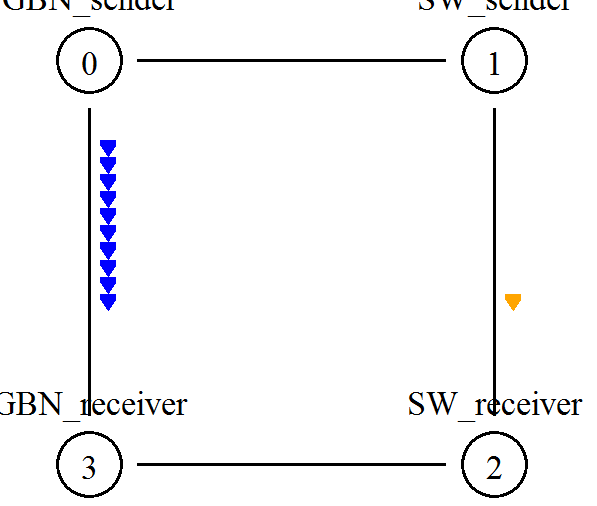
\includegraphics[width=0.40\textwidth]{8.png}
	\label{fig:8}
\end{figure}
\newpage
\textbf{\textsl{Απαντήσεις Ερωτήσεων}}
\begin{itemize}
\item Με τη βοήθεια του $NAM$, εντοπίστε τη χρονική στιγμή που ολοκληρώνεται η μετάδοση των 100
πακέτων $FTP$ στην περίπτωση του πρωτοκόλλου: (i) \textlatin{Go back N} και (ii) \textlatin{Stop and Wait}.\\
\underline{Απάντηση} : Για την περίπτωση του πρωτοκόλλου \textlatin{Go back N} η μετάδοση των 100 μπλε πακέτων ολοκληρώνεται τη χρονική στιγμή $t=1.211615$ $sec$. Αυτό προκύπτει από την προσομοίωση στο $NAM$ , στην οποία στέλνονται 10 ομάδες των 10 πακέτων ( μιας και το μέγεθος παραθύρου είναι 10) και καταγράψαμε τη χρονική στιγμή που έφτασε το τελευταίο πακέτο από την τελευταία ομάδα στον αποδέκτη 3. Επίσης, από το \textlatin{animation} βλέπουμε πως η αποστολή  των πρωτοκόλλων επιβεβαίωσης στον πομπό 0 των 10 τελευταίων πακέτων ολοκληρώνεται τη χρονική στιγμή $t=1.262173$ $sec$.\\
Για την περίπτωση του πρωτοκόλλου \textlatin{Stop and Wait} , βλέπουμε πως αποστέλλονται κάθε φορά ομάδες του ενός πακέτου ( μιας και το μέγεθος παραθύρου είναι 1). Η μετάδοση των 100 πακέτων ολοκληρώνεται τη χρονική στιγμή : $t=10.077776$ $sec$, ενώ τα πρωτοκόλλα επιβεβαίωσης του τελευταίου πακέτου στον πομπό 1 φτάνουν τη χρονική στιγμή $t=10.129602$ $sec$.
\item Ποιο είναι το ελάχιστο μέγεθος παραθύρου εκπομπής ($Nopt$) που εξασφαλίζει ελάχιστο χρόνο
μετάδοσης του συνόλου των πακέτων στο πρωτόκολλο \textlatin{Go back N} $?$\\
\underline{Απάντηση} : H χωρητικότητα της ζεύξης ισούται με : $\frac{max\_bandwidth}{delay}= \frac{3Mbps}{48ms}= 144000 bits = 18000 bytes$. Επίσης , το μέγεθος του πακέτου είναι $960+40=1000$ $bytes$ ( μαζί με την επικεφαλίδα των 40 $bytes$ ). Άρα, κάθε στιγμή στη ζεύξη χωράνε $\frac{18000}{1000}=18$ πακέτα. Τώρα, πρέπει να αντιληφθούμε ότι για κάθε πακέτο , αποστέλλεται και ένα αντίστοιχο πρωτόκολλο από τον δέκτη στον πομπό , αφού πρώτα σταλεί το πακέτο πληροφορίας στον δέκτη. Μπορούμε, συνεπώς να δούμε ότι το ελάχιστο μέγεθος παραθύρου είναι $N=2*18 + 1 = 37$ πακέτα , όπου ο άσος προστίθεται ακριβώς γι' αυτή την καθυστέρηση μεταξύ αποστολής πακέτου και πρωτοκόλλου. 
\item Με βάση το ελάχιστο αυτό μέγεθος παραθύρου που προσδιορίσατε στο προηγούμενο ερώτημα, τροποποιήστε τις εντολές
\selectlanguage{english}
\begin{verbatim}
$tcp0 set window_ X
$tcp0 set windowInit_ X
\end{verbatim}
\selectlanguage{greek}

εκτελέστε την προσομοίωση και υπολογίστε τη χρονική στιγμή που ολοκληρώνεται η μετάδοση
των 100 πακέτων $FTP$ για το πρωτόκολλο \textlatin{Go back N} με τη βοήθεια του $NAM$.\\
\underline{Απάντηση}  : Αλλάζουμε τις συγκεκριμένες εντολές του κώδικα σε :
\selectlanguage{english}
\begin{verbatim}
$tcp0 set window_ 37
$tcp0 set windowInit_ 37
\end{verbatim}
\selectlanguage{greek}
Με την αλλαγή του μεγέθους παραθύρου βλέπουμε πως η χρονική στιγμή αποστολής του τελευταίου πακέτου τώρα είναι $t=0.564048$ $sec$, ενώ το τελευταίο πακέτο πρωτοκόλλου επιβεβαίωσης φτάνει στον πομπό 0 τη στιγμή $t=0.613666$ $sec$.

\begin{figure}[htbp]
	\centering
		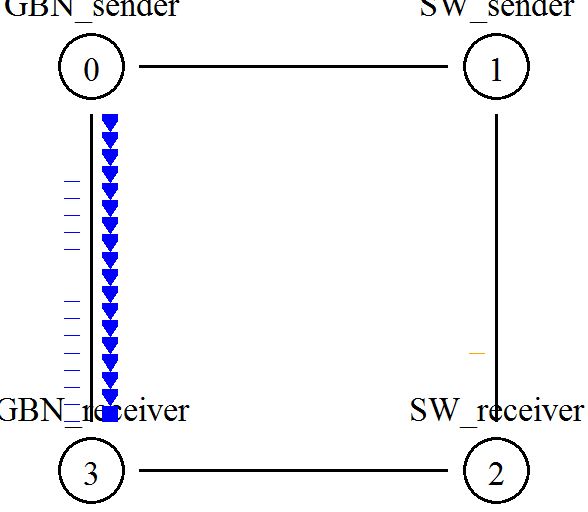
\includegraphics[width=0.30\textwidth]{1.png}
	\label{fig:1}
	\caption{ Αποστολή 37 πακέτων με $GBN$}
\end{figure}

\item Πόση είναι η μέγιστη καθυστέρηση διάδοσης της ζεύξης $n(0)-n(3)$ ώστε το αρχικό μέγεθος
παραθύρου ($Ν=10$) να οδηγεί σε συνεχή χρησιμοποίηση της ζεύξης (\textlatin{no idle time})$?$\\
\underline{Απάντηση}  : Θα βρούμε ,αρχικά, τα πακέτα που πρέπει να χωράνε στη ζεύξη για να έχουμε συνεχή χρησιμοποίηση της ζεύξης. Άρα, $2*N+1=10 \Rightarrow N= 4.5$ πακέτα. Συνεπώς, η μέγιστη καθυστέρηση της ζεύξης προκύπτει ότι η μέγιστη καθυστέρηση της ζεύξης είναι $\frac{3Mbps}{1000 bytes} =  12 ms$.
\item Εκτελέστε πάλι την προσομοίωση με το μέγεθος παραθύρου του πρωτοκόλλου \textlatin{Go back N} που
βρήκατε στο δεύτερο ερώτημα ($Nopt$), όταν η ζεύξη $n(0)-n(3)$ έχει διπλάσια και υποτριπλάσια
καθυστέρηση διάδοσης της αρχικής. Εντοπίστε τη χρονική στιγμή που ολοκληρώνεται η μετάδοση
των 100 πακέτων $FTP$ στον κόμβο $n3$ στις δύο αυτές περιπτώσεις. Τι παρατηρείτε $?$\\
\underline{Απάντηση} : Αρχικά , αλλάζουμε την καθυστέρηση διάδοσης σε διπλάσια της αρχικής : $48*2=96ms$. Βρίσκουμε πως το τελευταίο πακέτο από τα 100 φτάνει στον κόμβο 3 τη χρονική στιγμή : $t=0.8012$ $sec$. Ο χρόνος , δηλαδή έχει μεγαλώσει και επίσης, δέν έχουμε συνεχή χρησιμοποίηση της ζεύξης.Αν αλλάξουμε την καθυστέρηση διάδοσης σε υποτριπλάσια παρατηρούμε πως το τελευταίο πακέτο φτάνει τη χρονική στιγμή : $t=0.53348$ $sec$. Ο χρόνος , δηλαδή μειώθηκε σε σχέση με τον αρχικό , κάτι που οφείλεται στο ότι διατηρείται η πλήρης χρησιμοποίηση της ζεύξης. Παρακάτω , φαίνονται οι δύο περιπτώσεις :

\begin{figure}[htbp]
\centering
\begin{minipage}{0.49\textwidth}
\centering
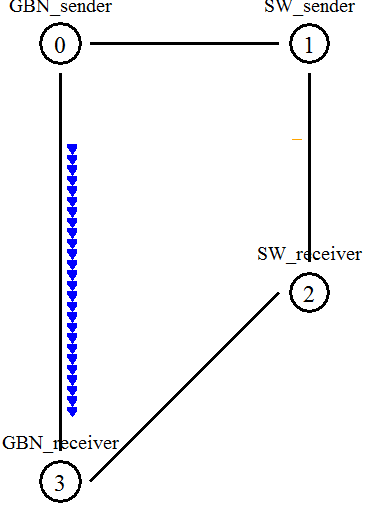
\includegraphics[width=0.30\textwidth]{2.png}
\caption{α) $t=96ms$}
\end{minipage}\hfill
\begin{minipage}{0.49\textwidth}
\centering
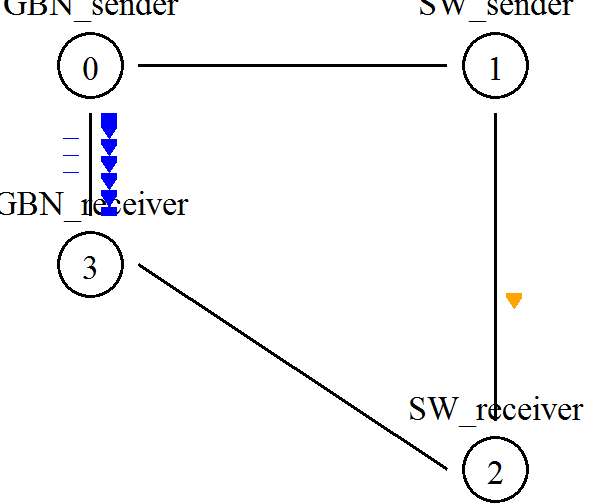
\includegraphics[width=0.50\textwidth]{3.png}
\caption{β) $t=16ms$}
\end{minipage}
\end{figure}


\end{itemize}

\section{Ανάλυση αποτελεσμάτων με τη βοήθεια του αρχείου ίχνους (\textlatin{trace file})}



\textbf{\textsl{Απαντήσεις Ερωτήσεων}}
\begin{itemize}
\item Ποιος είναι ο αριθμός των πακέτων που παρελήφθησαν, πόσα δεδομένα παρελήφθησαν από τον
παραλήπτη κατά τη διάρκεια της προσομοίωσης για κάθε ροή κίνησης $?$\\
\underline{Απάντηση} : Για τη συγκεκριμένη άσκηση έχουμε καθυστέρηση ζεύξης ίση με $d=110ms$. Επίσης , θέσαμε ως χρόνο προσομοίωσης $t=30sec$, για να προλάβουν να μεταδοθούν τα πακέτα.\\\\
Για $N=10$ προέκυψαν τα παρακάτω δεδομένα:
\begin{figure}[htbp]
	\centering
		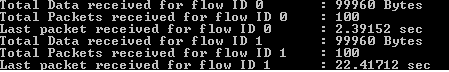
\includegraphics[width=1.00\textwidth]{5.png}
	\label{fig:5}
\end{figure}\\
Για $N=37$ προέκυψαν τα παρακάτω :
\begin{figure}[htbp]
	\centering
		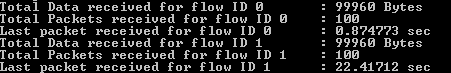
\includegraphics[width=1.00\textwidth]{4.png}
	\label{fig:4}
\end{figure}
\item Εξετάζοντας το αρχείο ίχνους, προσδιορίστε σε πόσο χρόνο απεστάλησαν αυτά τα δεδομένα στις
δύο περιπτώσεις για κάθε ροή κίνησης. Ποιος ο μέσος ρυθμός μετάδοσης δεδομένων σε $bps$ και
ποια είναι η χρησιμοποίηση του καναλιού $?$\\

\underline{Απάντηση} : Για την περίπτωση $N=10$ έχουμε :\\
Από τα αποτελέσματα που μας προέκυψαν από το αρχείο $awk$ έχουμε πως για τα πρωτόκολλα $GBN$ η αποστολή των πακέτων ολοκληρώνεται σε : $t=2.39152-0.25=2.14152$ $sec$. Άρα, ο μέσος ρυθμός μετάδοσης είναι : $\frac{99960*8}{2.14152}=373417.0122$ $bps$ και η χρησιμοποίηση είναι $\frac{373417.0122}{3000000}=12.447\%$. Για το πρωτόκολλο $SW$ η αποστολή πακέτων ολοκληρώνεται σε $t=22.527227-0.25=22.277227$ $sec$. Άρα, ο μέσος ρυθμός μετάδοσης είναι : $\frac{99960*8}{22.277227}=35896.74783$ $bps$ και η χρησιμοποίηση είναι $\frac{35896.7}{3000000}=1.1\%$.\\
Αντίστοιχα ,για την περίπτωση $N=37$ έχουμε : \\ 
Από τα αποτελέσματα που μας προέκυψαν από το αρχείο $awk$ έχουμε πως για τα πρωτόκολλα $GBN$ η αποστολή των πακέτων ολοκληρώνεται σε : $t=0.874773-0.25=0.624773$ $sec$. Άρα, ο μέσος ρυθμός μετάδοσης είναι : $\frac{99960*8}{0.624773}=1279952.879$ $bps$ και η χρησιμοποίηση είναι $\frac{1279952.879}{3000000}=42.66\%$.Για το πρωτόκολλο $SW$ η αποστολή πακέτων ολοκληρώνεται σε $t=22.527227-0.25=22.277227$ $sec$. Άρα, ο μέσος ρυθμός μετάδοσης είναι : $\frac{99960*8}{22.277227}=35896.74783$ $bps$ και η χρησιμοποίηση είναι $\frac{35896.7}{3000000}=1.1\%$.\\
\item Τροποποιείστε το $script$ ώστε να υπολογίσετε το χρόνο λήψης της επιβεβαίωσης (τύπος πακέτου
$ack$) του τελευταίου πακέτου στις δύο περιπτώσεις για κάθε ροή κίνησης. Επισυνάψτε στην
απάντησή σας και το τροποποιημένο $script$.\\
\underline{Απάντηση} : Παρακάτω, βρίσκονται τα αποτελέσματα και ο τροποποιήμενος κώδικας :
Για $N=10$:
\begin{figure}[htbp]
	\centering
		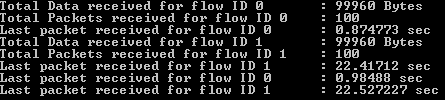
\includegraphics[width=1.00\textwidth]{6.png}
	\label{fig:6}
\end{figure}


και για $N=37$:
\begin{figure}[htbp]
	\centering
		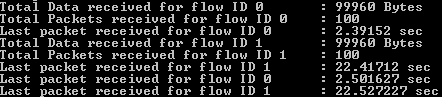
\includegraphics[width=1.00\textwidth]{7.png}
	\label{fig:7}
\end{figure}
και τέλος ο κώδικας :
\selectlanguage{english}
\begin{verbatim}
BEGIN {
 data_0=0;
 packets_0=0;
 data_1=0;
 packets_1=0;
}
/^r/&&/tcp/ {
 flow_id = $8;
 if (flow_id == 0) {
 data_0 += $6;
 packets_0++;
 last_ts_0 = $2;
 }
 if (flow_id == 1) {
 data_1 += $6;
 packets_1++;
 last_ts_1 = $2;
 }
}

/^r/&&/ack/ {
 flow_id = $8;
 if (flow_id == 0) {
 last_ack_0=$2;
 }
 if (flow_id == 1) {
 last_ack_1=$2;
 }
}

END {
 printf("Total Data received for flow ID 0\t: %d Bytes\n", data_0);
 printf("Total Packets received for flow ID 0\t: %d\n", packets_0);
 printf("Last packet received for flow ID 0\t: %s sec\n", last_ts_0);
 printf("Total Data received for flow ID 1\t: %d Bytes\n", data_1);
 printf("Total Packets received for flow ID 1\t: %d\n", packets_1);
 printf("Last packet received for flow ID 1\t: %s sec\n", last_ts_1);
 printf("Last packet received for flow ID 0\t: %s sec\n", last_ack_0);
 printf("Last packet received for flow ID 1\t: %s sec\n", last_ack_1);

}
\end{verbatim}

\end{itemize}



\end{document}